 %%%%%%%%%%%%%%%%%%%%%%%%%%%%%%%%%%%%%%%%
% datoteka diploma-vzorec.tex
%
% vzorčna datoteka za pisanje diplomskega dela v formatu LaTeX
% na UL Fakulteti za računalništvo in informatiko
%
% vkup spravil Gašper Fijavž, december 2010
% množica popravkov v januarju, februarju marcu 2011
% verzija 29. marec 2011

\documentclass[a4paper, 12pt]{book}

\usepackage[utf8x]{inputenc}   % omogoča uporabo slovenskih črk kodiranih v formatu UTF-8 
\usepackage[slovene,english]{babel}    % naloži, med drugim, slovenske delilne vzorce
\usepackage[pdftex]{graphicx}  % omogoča vlaganje slik različnih formatov 
\usepackage{fancyhdr}          % poskrbi, na primer, za glave strani
\usepackage{amssymb}           % dodatni simboli
\usepackage{amsmath}           % eqref, npr.
\usepackage[boxed]{algorithm2e}
\usepackage{mathtools}
\usepackage{listings}
\usepackage{color}
\usepackage{amssymb}

\renewcommand{\algorithmcfname}{Algoritem}
\renewcommand{\baselinestretch}{1.3} % ustrezen razmik med vrsticami

%oznake strani
\renewcommand{\chaptermark}[1]%
{\markboth{\MakeUppercase{\thechapter.\ #1}}{}} \renewcommand{\sectionmark}[1]%
{\markright{\MakeUppercase{\thesection.\ #1}}} \renewcommand{\headrulewidth}{0.5pt} \renewcommand{\footrulewidth}{0pt} 
\fancyhf{}
\fancyhead[LE,RO]{\sl \thepage} \fancyhead[LO]{\sl \rightmark} \fancyhead[RE]{\sl \leftmark}

\newcommand{\BibTeX}{{\sc Bib}\TeX}

\newcommand{\autfont}{\Large}
\newcommand{\titfont}{\LARGE\bf}
\newcommand{\clearemptydoublepage}{\newpage{\pagestyle{empty}\cleardoublepage}}
\setcounter{tocdepth}{1}	      % globina kazala

% konstrukti
\newtheorem{izrek}{Izrek}[chapter]
%\newtheorem{trditev}{Trditev}[izrek]
\newenvironment{dokaz}{\emph{Dokaz.}\ }{\hspace{\fill}{$\Box$}}

 \raggedbottom
\begin{document}
\selectlanguage{slovene}
\frontmatter
\setcounter{page}{1} %
\renewcommand{\thepage}{}       % preprecimo težave s številkami strani v kazalu 

%%%%%%%%%%%%%%%%%%%%%%%%%%%%%%%%%%%%%%%%
%naslovnica
 \thispagestyle{empty}%
   \begin{center}
    {\large\sc Univerza v Ljubljani\\%
      Fakulteta za ra\v cunalni\v stvo in informatiko}%
    \vskip 10em%
    {\autfont Simon Ivan\v sek\par}%
    {\titfont Vizualizacija optimizacije prometa z genetskimi algoritmi \par}%
    {\vskip 2em \textsc{DIPLOMSKO DELO\\[2mm] 
    VISOKO\v SOLSKI STROKOVNI \v STUDIJSKI PROGRAM PRVE STOPNJE RA\v CUNALNI\v STVO IN INFORMATIKA}\par}%
    \vfill\null%
    {\large \textsc{Mentor}: prof.\ dr.  Marko Robnik \v Sikonja\par}%
    {\vskip 2em \large Ljubljana 2012 \par}%
\end{center}
% prazna stran
\clearemptydoublepage

%%%%%%%%%%%%%%%%%%%%%%%%%%%%%%%%%%%%%%%%
%copyright stran
\thispagestyle{empty}
\vspace*{8cm}
{\small \noindent
Rezultati diplomskega dela so intelektualna lastnina avtorja in Fakultete za ra\-\v cu\-nal\-ni\v s\-tvo in informatiko Univerze v Ljubljani. 
Za objavljanje ali izkori\v s\v canje rezultatov di\-plom\-ske\-ga dela je potrebno pisno soglasje avtorja, Fakultete za ra\-\v cu\-nal\-ni\v s\-tvo in 
informatiko ter mentorja.}

\begin{center} 
\mbox{}\vfill
\emph{Besedilo je oblikovano z urejevalnikom besedil \LaTeX.} 
\end{center}
% prazna stran
\clearemptydoublepage

%%%%%%%%%%%%%%%%%%%%%%%%%%%%%%%%%%%%%%%%
% stran 3 med uvodnimi listi
\noindent
Namesto te strani {\bf vstavite} original izdane teme diplomskega 
dela s podpisom mentorja in dekana ter žigom fakultete, ki ga diplomant
dvigne v študent\-skem referatu,  preden odda izdelek v vezavo!
Glej tudi sam konec Poglavja~\ref{ch2} na strani~\pageref{pp}.

% prazna stran
\clearemptydoublepage

%%%%%%%%%%%%%%%%%%%%%%%%%%%%%%%%%%%%%%%%
% izjava o avtorstvu
\vspace*{1cm}
\begin{center} 
{\Large \textbf{\sc Izjava o avtorstvu diplomskega dela}}
\end{center}

\vspace{1cm}
\noindent Spodaj podpisani Simon Ivan\v sek,
z vpisno \v stevilko \textbf{63080273}, sem avtor  diplomskega dela z naslovom:
   
\vspace{0.5cm}
\emph{Vizualizacija optimizacije prometa z genetskimi algoritmi}

\vspace{1.5cm}
\noindent S svojim podpisom zagotavljam, da:
\begin{itemize}
	\item sem diplomsko delo izdelal samostojno pod mentorstvom 
		prof.\ dr.\ Marka Robnik \v Sikonje

	\item	so elektronska oblika diplomskega dela, naslov, povzetek, ter klju\v cne besede identi\v cni s tiskano obliko diplomskega dela
	\item sogla\v sam z javno objavo elektronske oblike diplomskega dela v zbirki ''Dela FRI''.
\end{itemize}

\vspace{1cm}
\noindent V Ljubljani, dne 15. avgusta 2012 \hfill Podpis avtorja:

% prazna stran
\clearemptydoublepage

%%%%%%%%%%%%%%%%%%%%%%%%%%%%%%%%%%%%%%%%
% zahvala
\thispagestyle{empty}\mbox{}\vfill\null\it
Zahvalil bi se mentorju prof. dr. Marku Robnik \v Sikonji za koristne nasvete in vso izkazano podporo med izdelavo diplomskega dela.

Zahvalil bi se tudi direktorju podjetja Xlab d.o.o., ki mi je kljub moji navzo\v cnosti v podjetju omogo\v cil nemoteno in kakovostno okolje za izdelavo diplomskega dela.
\rm\normalfont
 
% prazna stran
\clearemptydoublepage

%%%%%%%%%%%%%%%%%%%%%%%%%%%%%%%%%%%%%%%%
% kazalo
\def\thepage{}% preprecimo tezave s stevilkami strani v kazalu 
\tableofcontents{}


% prazna stran
\clearemptydoublepage

%%%%%%%%%%%%%%%%%%%%%%%%%%%%%%%%%%%%%%%%
% povzetek 
\addcontentsline{toc}{chapter}{Povzetek}
\chapter*{Povzetek}
Cilj diplomske naloge je priprava u\v cnega pripomo\v cka za pou\v cevanje genetskih algoritmov. Implementirali smo ga kot spletno stran, genetske algoritme pa uporabili za optimizacijo prometa. Optimizacijo prometa smo zastavili kot optimizacijo \v casa rde\v cih in zelenih lu\v ci na semaforjih tako, da vozila v cestnem omre\v zju prevozijo obravnavani segment cestnega omre\v zja kar najhitreje. Cestno omre\v zje smo definirali kot graf, za iskanje najkraj\v se poti v grafu smo uporabili algoritem Dijkstra. Kon\v cne nastavitve \v casov rde\v cih in zelenih lu\v ci za vsa kri\v zi\v s\v ca v cestnem omre\v zju, smo vizualizirali z animacijo prometa in analizo uspe\v snosti optimizacije.

% prazna stran
\clearemptydoublepage

%%%%%%%%%%%%%%%%%%%%%%%%%%%%%%%%%%%%%%%%
% abstract
\selectlanguage{english}
\addcontentsline{toc}{chapter}{Abstract}
\chapter*{Abstract}
In this thesis we prepare a learning tool for genetic algorithms. We implemented it as a web site where genetic algorithms solve a traffic optimization problem. The traffic optimization problem is defined as timing of red and green traffic lights for traffic in a given road network segment to flow as fast as possible. Road network is presented as graph and the shortest paths in graph are found with Dijkstra algorithm. Final configurations of red and green light timings for all intersections in the road segment are visualized with traffic animation and analysis of optimization.

\selectlanguage{slovene}
% prazna stran
\clearemptydoublepage

%%%%%%%%%%%%%%%%%%%%%%%%%%%%%%%%%%%%%%%%
\mainmatter
\setcounter{page}{1}
\pagestyle{fancy}

\chapter{Uvod}
\label{ch1}
%Genetski algoritmi posnemajo proces naravne evolucije in se rutinsko uporabljajo za generiranje uporabnih re\v sitev pri optimizaciji in iskanju. Pripadajo skupini, t.i. evolucijskih algoritmov in generirajo re\v sitve z uporabo tehnik evolucije, kot so dedovanje, mutacija, izbira in kri\v zanje. 
%\cite{wikipedia genetski algoritmi}

S hitrim razvojem ekonomije in porastom prebivalstva so prometni zastoji postali eden resnej\v sih problemov v ve\v cjih mestih. V preteklosti so take probleme re\v sevali z dodajanjem pasov in novih povezav v \v ze obstoje\v ca omre\v zja. Z razvojem tehnologije pa so tudi semaforji postali bolj inteligentni in se prilagajajo trenutnemu prometu. 
Ponavadi so kri\v zi\v s\v ca  in neusklajeni \v casi lu\v ci na semaforjih glavni vzrok za zastoje na cestah zato je pomembno, kako dolo\v cimo \v case rde\v cih in zelenih lu\v ci. 
\cite{he12-aes.pdf}

Z dodajanjem kri\v zi\v s\v c in semaforjev nara\v s\v ca zahtevnost optimizacije prometa. Klasi\v cne deterministi\v cne postopke je te\v zko uporabiti na problemih z visoko zahtevnostjo, saj pogosto niso \v casovno sprejemljivi. Genetski algoritmi, s posnemanjem procesa evolucije, delujejo \v casovno bolj sprejemljivo, vendar ne zagotavljajo optimalnosti.

Z genetskimi algoritmi \v zelimo optimizirati \v case rde\v cih in zelenih lu\v ci na semaforjih tako, da vsa vozila pridejo od za\v cetka do cilja \v cimhitreje in po najkraj\v si poti. Re\v sitve vizualiziramo z animacijo premikanja vozil v cestnem omre\v zju s semaforji in kri\v zi\v s\v ci. Cestno omre\v zje vnaprej definiramo, \v stevilo vozil pa je parameter. Animacija poteka toliko \v casa, da vsi avtomobili prispejo na cilj. Animacija slu\v zi kot orodje za la\v zjo razlago delovanja genetskih algoritmov na realnem problemu.

\section{Napoved vsebine po poglavjih}
\textbf{V drugem poglavju} opi\v semo delovanje genetskih algoritmov, razlo\v zimo delovanje razli\v cnih genetskih operatorjev (kri\v zanje, mutacija) in opi\v semo razli\v cne metode izbire osebkov za reprodukcijo.\\
\textbf{V tretjem poglavju} opi\v semo problem urejanja prometa, razlo\v zimo kako smo pristopili k problemu in kako smo re\v sevanje problema implementirali z genetskimi algoritmi.\\
\textbf{V \v cetrtem poglavju} opi\v semo tehnologije uporabljene pri implementaciji genetskih algoritmov in animaciji.\\
\textbf{V petem poglavju} predstavimo in razlo\v zimo rezultate genetskih algoritmov.\\
\textbf{V zadnjem poglavju} predstavimo glavne ugotovitve in ideje za izbolj\v save.

\chapter{Genetski algoritmi}
\label{ch1}
Genetski algoritmi omogo\v cajo enostaven in skoraj generi\v cen pristop k re\v sevanju kompleksnih optimizacijskih problemov. Kljub enostavnosti genetski algoritem potrebuje smiselne in dolo\v cene parametre, da lahko najde dobre re\v sitve. Izbira neustreznih parametrov vodi v dalj\v si \v cas izvajanja programa in slab\v se rezultate
\cite{sarmady}.

V nadaljevanju opi\v semo predstavitev zna\v cilno za genetske algoritme, genetske operatorje kri\v zanja in mutacije, funkcijo kvalitete in nekaj postopkov za izbiro osebkov za reprodukcijo.
Delovanje genetskega algoritma prikazuje slika \ref{fig:izvajanje_ga}.
\begin{figure}
\begin{center}
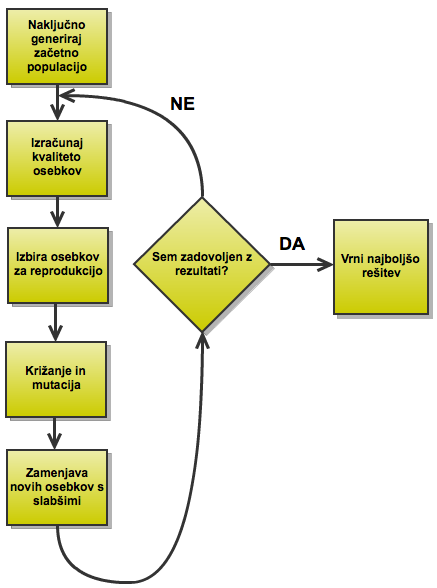
\includegraphics[scale=0.70]{izvajanje_ga.png}
\end{center}
\caption{Prikaz delovanja genetskega algoritma.}
\label{fig:izvajanje_ga}
\end{figure}

\section{Predstavitev osebkov}
\label{seq:predstavitev osebkov}
Za delo z genetskimi algoritmi moramo problem predstaviti v taki obliki, da lahko re\v sitvi dolo\v cimo kvaliteto in nad njo izvajamo genetske operatorje.
Predstavitvi ene re\v sitve pravimo \textbf{osebek}.

\subsection{Biolo\v sko ozadje}

Vsak organizem vsebuje mno\v zico pravil in na\v crt, ki opisuje, kako je organizem zgrajen. Ta pravila so zakodirana v \textit{genih} organizma, ki so povezani v dolg niz, ki se imenuje \textit{kromosom}. Vsak gen predstavlja eno lastnost organizma, npr. barva o\v ci ali barva las in \v se veliko drugih lastnosti
\cite{aijunkie}. Osebke lahko predstavimo na ve\v c na\v cinov:

\begin{itemize} \itemsep0em
\item z biti,
\item vektorji
\item nizi,
\item drevesi, itd.
\end{itemize}

Osebek mora biti predstavljen tako, da mu je mogo\v ce dolo\v citi kvaliteto, saj glede na izra\v cunano kakovost, izberemo najbolj\v se med osebki in iz njih ustvarimo nove osebke.

Za na\v s problem je osebek predstavljen kot zaporedje parov \v casov rde\v cih in zelenih lu\v ci na semaforjih. Primer za pet kri\v zi\v s\v c bi zgledal takole:
\begin{center}
(20, 30), (60, 80), (10, 50), (50, 80), (10, 70)
\end{center}

En par \v stevil ustreza enemu kri\v zi\v s\v cu, \v casi pa so v sekundah in predstavljajo dele\v z sekunde. Par (20, 30) pomeni, da rde\v ca lu\v c gori 20 sekund, zelena pa 30 sekund.

\section{Za\v cetna populacija}
Populacija je v terminologiji genetskih algoritmov mno\v zica osebkov. Za\v cetna populacija je lahko generirana naklju\v cno ali stohasti\v con, nato pa se z genetskimi operatorji spreminja.

Ve\v cja populacija izbolj\v suje delovanje genetskih algoritmov, vpliva pa tudi na \v stevilo generacij, potrebnih, da kvaliteta re\v sitev konvergira. Velikost populacije je odvisna od vrste problema, ponavadi vsebuje ve\v c sto ali tiso\v c osebkov.

\section{Funkcija kvalitete}
Funkcija kvalitete (ang. \textit{fitness function}) je funkcija, ki objektivno oceni, kako blizu cilja je neka re\v sitev.

Razlog, da genetski algoritmi niso trivialen na\v cin re\v sevanja problemov, je predvsem v energiji vlo\v zeni v oblikovanje delujo\v ce funkcije kvalitete. \v Ce je funkcija kvalitete oblikovana napa\v cno, bo algoritem konvergiral k napa\v cnim re\v sitvam, ali pa sploh ne bo konvergiral.\\\\
Znaki da je funkcija kvalitete slabo oblikovana so:
\begin{itemize}
\item \v cas ra\v cunanja kvalitete re\v sitve je velik,
\item natan\v cen model za izra\v cun kvalitete manjka.
\end{itemize}

\section{Kri\v zanje}
\label{seq:krizanje}
Kri\v zanje (\textit{ang. crossover}) je najpomembnej\v sa tehnika izmenjave genetskega materiala med osebki. Uporablja se eno, dvo in ve\v cmestno kri\v zanje. Enomestno kri\v zanje poteka tako, da naklju\v cno izberemo to\v cko kri\v zanja in preko te to\v cke izmenjamo genetski material (slika \ref{krizanje}).
\begin{figure}
\begin{center}
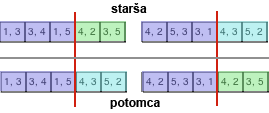
\includegraphics[scale=0.75]{krizanje.png}
\end{center}
\caption{Mesto kri\v zanja je ozna\v ceno z rde\v co \v crto. Prvi del (vijol\v cna barva) genetskega zapisa se ohrani, drugi del (zelena in turkizna barva) pa se izmenjata.}
\label{krizanje}
\end{figure}

Kri\v zanje naj bi generiralo bolj\v se osebke, saj naj bi se dobri deli genetskega zapisa ohranili in prenesli na potomce \cite{inteligentni sistemi}.

\section{Mutacija}
Mutacija je postopek, ko na nekem naklju\v cno izbranem mestu spremenimo genetski zapis izbranega osebka. 
Brez mutacij bi kri\v zanje lahko izmenjevalo samo genetski material vsebovan v za\v cetni slu\v cajno generirani generaciji osebkov. Mutacija doda potencialno novo informacijo. Verjetnost mutacije kljub njeni koristnosti ne sme biti prevelika, saj se sicer pokvari preve\v c koristnih genov v osebkih in postane evolucijsko ra\v cunanje podobno naklju\v cnemu preiskovanju
\cite{inteligentni sistemi}.

\section{Evolucijski model}
Evolucijski model imenujemo izbiro osebkov za razmno\v zevanje.
Osebke \v zelimo izbrati tako, da se dobri osebki, ki vsebujejo kakovosten genetski material, prenesejo v naslednjo generacijo. Zato je smiselno, da dobri osebki tvorijo ve\v c potomcev in da se morda celo nespremenjeni prenesejo v naslednjo generacijo. Slednje imenujemo elitelizem \cite{inteligentni sistemi}. Nekaj uveljavljenih evolucijskih modelov je predstavljenih v nadaljevanju.

\subsection{Proporcionalna izbira}
\label{seq:ruletno kolo}
Vsakemu osebku je dodeljena verjetnost izbire glede na njegovo kvaliteto. Naslednja ena\v cba prikazuje, kako je dodeljena verjetnost izbire $p_i$:

\begin{equation}
p_i = \frac{f_i}{\sum_{j=1}^n f_j}
\label{eq:proporcionalna izbira}
\end{equation}
Osebki so nato izbrani za reprodukcijo s pomo\v cjo metode ruletnega kolesa. Dele\v z kolesa, ki ga osebek zaseda, je sorazmeren njegovi uspe\v snosti. Izbiro z metodo ruletnega kolesa na populaciji velikosti 5 osebkov ilustrira slika \ref{ruletno kolo}.

\begin{figure}[h]
\begin{center}
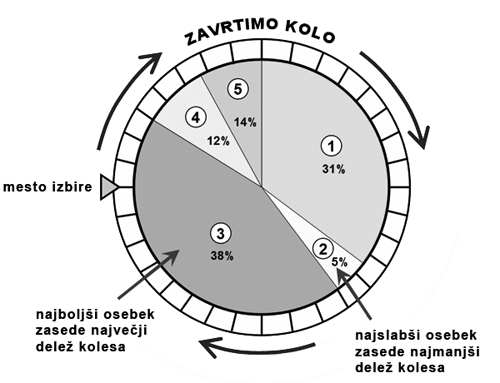
\includegraphics[scale=0.65]{ruletno_kolo.png}
\end{center}
\caption{Izbira osebkov za reprodukcijo z metodo ruletnega kolesa. Osebek zaseda dele\v z kolesa proporcionalen njegovi kvaliteti \cite{slika ruletno kolo}.}
\label{ruletno kolo}
\end{figure}
Slabost tak\v snega na\v cina izbire je, da lahko dobri osebki zelo hitro prevladajo, \v ze po nekaj generacijah, ker vsaki\v c zasedajo ve\v cji dele\v z ruletnega kolesa.

Druga slabost izbire z ruletnim kolesom je, da \textbf{ne deluje} za probleme, kjer \v zelimo kvaliteto osebkov minimizirati. Te\v zavo odpravimo tako, da problem minimizacije kvalitete prevedemo na problem maksimizacije kvalitete z ustreznimi transformacijami.

\subsection{Enoturnirska izbira}
Enoturnirska izbira je eden izmed na\v cinov turnirske izbire. Gre za priljubljen in preprost na\v cin hkratne izbire osebkov za razmno\v zevanje in isto\v casno nadome\v s\v canja osebkov. Poteka takole:
\begin{enumerate}
\item naklju\v cno razbij populacijo na majhne skupine velikosti \textit{g},
\item dva najbolj\v sa osebka iz vsake skupine se kri\v zata in njuna potomca nadomestita najslab\v sa osebka v skupini.
\end{enumerate}

Prednost enoturnirske izbire je, da pre\v zivi v naslednjo generacijo (\textit{g - 2}) najbolj\v sih osebkov in tako ne izgubljamo prehitro dobrih osebkov pa tudi maksimalna kvaliteta populacije ne pada. Po drugi strani strategija zagotavlja, da \v se tako dober osebek nima ve\v c kot dveh potomcev, in se tako ohranja raznolikost populacije
\cite{inteligentni sistemi}.

\subsection{Stohasti\v cno univerzalno vzor\v cenje}
Slabost do sedaj opisanih metod izbire je velika varianca glede na funkcijo kvalitete. Pri nekaterih evolucijskih modelih se lahko zgodi, da najbolj\v si osebek nima nobenega potomca. Manj\v so varianco zagotavlja stohasti\v cno univerzalno vzor\v cenje, ki ga ilustrira slika \ref{fig:stohasticno univerzalno vzorcenje}.

\begin{figure}
\begin{center}
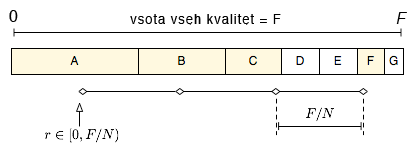
\includegraphics[scale=0.75]{stohasticno_univerzalno_vzorcenje.png}
\end{center}
\caption{Ilustracija stohasti\v cnega univerzalnega vzor\v cenja. Osebke razvrstimo na interval $[0, 1]$ proporcionalno njihovi kvaliteti. Izbiramo $N$ osebkov, zato za\v cetno to\v cko $r$ naklju\v cno izberemo na intervalu $[0, \frac{1}{N}]$. Osebke izberemo na mestih $r + \frac{i}{N}, i \in [0, 1, \dots, N-1]$ \cite{inteligentni sistemi}.}
\label{fig:stohasticno univerzalno vzorcenje}
\end{figure}

Na podlagi kvalitete osebka $f_i$ tvorimo verjetnostno distribucijo kot pri proporcionalni izbiri
$p_i = \frac{f_i}{\sum_{j=1}^n f_j}$. Osebke naklju\v cno razvrstimo na \v stevilski trak na interval med 0 in 1 in vsak dobi dol\v zino traku sorazmerno $p_i$. Dolo\v cimo \v stevilo osebkov N, ki jih \v zelimo generirati in naklju\v cno izberemo \v stevilo z intervala $[0, 1/N]$. Za razmno\v zevanje izberemo osebke, ki pokrivajo to\v cke $r + iN, i \in [0, 1, \dots, N -1]$ \cite{inteligentni sistemi}.

\section{Elitizem}
Elitizem je strategija, ki dolo\v cen del najbolj\v sih osebkov prenese direktno v naslednjo generacijo. Dobra stran te strategije je, da imamo v vsaki generaciji na voljo najbolj\v se osebke in jih ni potrebno posebej hraniti, poleg tega pa zaradi variance pri izbiri ne izgubljamo dobrega genetskega materiala. Slabost je v mogo\v ci prezgodnji konvergenci, \v ce elita prevlada
\cite{inteligentni sistemi}.

\chapter{Problem optimizacije prometa}
\label{ch2}
V tem poglavju predstavimo raziskave na podro\v cju optimizacije prometa, opi\v semo na\v s pristop k re\v sevanju problema in ga formaliziramo. Predstavimo algoritem za iskanje najkra\v se poti v grafu in uporabo genetskih algoritmov na problemu optimizacije prometa.

\section{Ozadje}
Promet na cestah se pove\v cuje s hitrej\v sim tempom kot porast prebivalstva. Problem urejanja prometa je prisoten v vseh ve\v cjih mestih v vseh dr\v zavah. Ve\v canje prometa povzro\v ca prometne zastoje, zato se vozniki in potniki sre\v cujejo s problemi, kot so nepotrebno zapravljanje \v casa, stresom, onesna\v zevanjem, pove\v cano nevarnostjo nesre\v c in ostalimi resnimi problemi. Obstajajo razli\v cni pristopi kako re\v sevati take probleme. Ena od mo\v znosti je uporaba obstoje\v cih cest s pravilnim rokovanjem semaforjev. 

Dana\v snje raziskave na podro\v cju optimizacije semaforjev lahko razdelimo na dva dela. Po eni strani je bilo veliko truda vlo\v zenega v razvoj visoko prilagodljivih semaforjev, ki so sposobni reagirati na spremembe v prometu takoj, v realnem \v casu. Po drugi strani, pa se ob delitvi \v casa na  faze (npr.: jutranja, popoldanska, no\v cna), zdi uporaba prednastavljenih semaforjev dokaj razumljiva.

Drugo razlikovanje bi lahko naredili med hevristi\v cnimi pristopi k optimizaciji in \v cistimi matemati\v cnimi pristopi in njihovimi osnovnimi modeli. Hevristi\v cni pristopi temeljijo na genetskih algoritmih, mehki logiki in nevronskih mre\v zah. Za njih je zna\v cilno da ponavadi dajejo dobre in hitre re\v sitve, ampak ne zagotavljajo  kvalitete dane re\v sitve v primerjavi z optimalno.

Matemati\v cni pristopi pa ponavadi ne morejo pokriti vseh zahtev in parametrov resni\v cnega cestnega omre\v zja, ampak ponujajo dokazano dobre re\v sitve. Take re\v sitve so lahko v\v casih dobre za\v cetne re\v sitve za hevristi\v cne pristope.

\section{Formalizacija problema}
Postavimo se v vlogo voznika, ki \v zeli priti od doma v slu\v zbo \v cimhitreje in po najkraj\v si poti skozi sredi\v s\v ce mesta, kjer je veliko semaforiziranih kri\v zi\v s\v c. Imamo \v se 19 prijateljev, nekateri \v zelijo priti od doma do trgovine, ki je na drugem koncu mesta, drugim pa se mudi v \v solo, a vsi \v zelijo priti na svoj cilj \v cimhitreje in po najkraj\v si poti. Potovalni \v cas vsakega vozila bo najkraj\v si takrat, ko bo najmanj \v casa \v cakal na rde\v cih lu\v ceh in v koloni ter bo \v sel po najkraj\v si poti
\footnote{Za iskanje najkraj\v se poti v grafu na sliki \ref{graph3} smo uporabili algoritem Dijkstra, opisan v razdelku \ref{seq:dijkstra}.}.

Cestno omre\v zje je predstavljeno z grafom $G = (V, E)$, kjer je $V$ mno\v zica vozli\v s\v c in $E$ mno\v zica ute\v zenih povezav med vozli\v s\v ci. Vozli\v s\v ca ustrezajo kri\v zi\v s\v cem, povezave pa cestam med kri\v zi\v s\v ci. Ute\v zi na povezavah ustrezajo razdalji (v metrih), ki jih mora vozilo prepotovati, da dose\v ze naslednje vozli\v s\v ce.  Dodatno zahtevamo, da je vozli\v s\v ce kri\v zi\v s\v ce, \v ce je njegova stopnja $>$ 2, sicer je vozli\v s\v ce bodisi za\v cetno bodisi kon\v cno. Vozilo lahko za\v cne in kon\v ca svojo pot le v kon\v cnih oziroma za\v cetnih vozli\v s\v cih. Slika \ref{graph3} v obliki grafa prikazuje mo\v zno postavitev cestnega omre\v zja.
\begin{figure}
\begin{center}
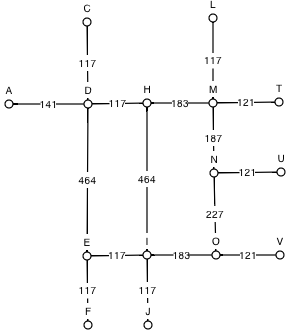
\includegraphics[totalheight=0.4\textheight]{graph3.png}
\end{center}
\caption{Primer grafa s 15 vozli\v s\v ci in ute\v zenimi povezavami med njimi.}
\label{graph3}
\end{figure}

\section{Iskanje najkraj\v se poti v grafih}
\label{seq:dijkstra}
Algoritem Dijkstra je zasnoval nizozemski ra\v cunalni\v ski in\v zenir Edsger Dijkstra. Algoritem poi\v s\v ce najkraj\v so pot v usmerjenem grafu z nenegativnimi ute\v zenimi povezavami. Za podano za\v cetno vozli\v s\v ce v grafu algoritem poi\v s\v ce najcenej\v so pot med za\v cetnim vozli\v s\v cem in vsemi ostalimi vozli\v s\v ci. Lahko ga uporabimo tudi za iskanje najcenej\v se poti med za\v cetnim vozli\v s\v cem in kon\v cnim vozli\v s\v cem. Primer take uporabe je na\v s graf na sliki \ref{graph3}.

\section{Genetski algoritem}
\label{seq:nastavitve parametrov}
V poglavju \ref{ch2} smo na splo\v sno opisali delovanje genetskih algoritmov. V tem razdelku pa opi\v semo, kako smo uporabili genetske algoritme na na\v sem problemu.

V nadaljevanju so na\v stete privzete nastavitve genetskih algoritmov in nastavitve animacije. Te nastavitve bomo uporabljali tudi v nadaljevanju, ko opisujemo, kako smo implementirali operacije genetskih algoritmov in pri predstavitvi rezultatov.\\\\
Nastavitve genetskih algoritmov:
\begin{itemize}
\item \v st. generacij = 100,
\item velikost populacije = 100,
\item dele\v z kri\v zanja = 0.70,
\item dele\v z mutacije = 0.05.
\end{itemize}
Nastavitve animacije:
\begin{itemize}
\item FPS = 50,
\item hitrost vozila = 50 $\frac{km}{h}$,
\item hitrost animacije = 20.
\end{itemize}
Hitrost animacije lahko spreminjamo na intervalu $[1, 20]$ s korakom 1.

Parameter \textit{FPS} (ang. \textit{frames per second}) in \textit{hitrost vozila} sta vnaprej definirana in ju uporabnik ne more spreminjati, vendar ju navajamo, saj sta pomembna za nadaljevanje.

\subsection{Funkcija kvalitete}
V razdelku \ref{seq:predstavitev osebkov} smo osebek predstavili kot zaporedje parov \v casov rde\v cih in zelenih lu\v ci na semaforjih, optimizacijski problem pa smo formalizirali na primeru 20 vozil.

Na\v s cilj je za vseh 20 vozil poiskati optimalno nastavitev \v casov rde\v cih in zelenih lu\v ci na semaforjih, tako da bodo vsa vozila pri\v sla na cilj \v cimprej. To pomeni, da moramo izra\v cunati ali izmeriti \v cas potovanja \textbf{vseh} vozil.

Kvaliteto re\v sitve ocenimo s simulacijo \footnote{Simulacijo smo izvedli enako kot animacijo, le da ni\v cesar ne izri\v semo.}, pri \v cemer smo parameter \textit{hitrost animacije} nastavili na vrednost 20 zato, da je simulacija hitrej\v sa. Simulacija simulira premikanje vseh vozil od za\v cetnega vozli\v s\v ca do kon\v cnega, pri tem pa merimo \v cas dokler vsa vozila ne pridejo na cilj. \textcolor{red}{Zaradi tehni\v cnih razlogov merimo \v stevilo korakov potrebnih za to, da vsa vozila prispejo na cilj. \v Stevilo korakov pretvorimo v \v cas potovanja z naslednjo formulo:}

\begin{equation}
\textcolor{red}{\textrm{\textit{\v cas potovanja}} = \frac{\textrm{\textit{prepotovana dol\v zina vseh vozil}}}{\textrm{\textit{hitrost vozila ($\frac{m}{s}$)}}}}
\end{equation}

\begin{equation}
\textcolor{red}{\textrm{\textit{prepotovana dol\v zina vseh vozil}} = \textrm{\textit{\v stevilo iteracij}}*\textrm{\textit{velikost koraka}}}
\label{eq:prepotovana dolzina}
\end{equation}

\begin{equation}
\textcolor{red}{\textrm{\textit{velikost koraka}} = \frac{\textrm{\textit{hitrost vozila}}*\textrm{\textit{hitrost animacije}}}{FPS}}
\label{eq:velikost koraka}
\end{equation}

\textcolor{red}{Velikost koraka (ena\v cba \ref{eq:velikost koraka}) slu\v zi za pretvorbo realne hitrosti vozila ($\frac{km}{h}$) v enoto potrebno za animacijo, oz. simulacijo ($\frac{px}{iteracijo}$).}

\subsection{Proporcionalna izbira}
Slabost izbire z ruletnim kolesom je, da ne deluje za minimizacijske probleme in moramo zato minimizacijski problem prevesti na maksimizacijski. V na\v sem primeru, kjer manj\v sa vrednost pomeni bolj\v so kvaliteto, smo to naredili tako, da predno kli\v cemo metodo ruletnega kolesa, zamenjamo kvalitete najslab\v sega z najbolj\v sim (tabela \ref{fig:zamenjava kvalitete}).\\ Po izvajanju metode zamenjamo kvalitete nazaj.

\begin{table}
\begin{center}
\begin{tabular}{l | c | r}
i & $f_i$ \\
\hline
4 & 87 \\
1 & 135 \\
2 & 213 \\
5 & 333 \\
3 & 413 \\
\end{tabular}
\hspace{6mm} $=>$ \hspace{6mm}
\begin{tabular}{l | c | r}
i & $f_i$ \\
\hline
4 & 413 \\
1 & 333 \\
2 & 213 \\
5 & 135 \\
3 & 87 \\
\end{tabular}
\end{center}
\caption{Zamenjava ocen kvalitet najslab\v sih (ve\v cja \v stevilka) z najbolj\v simi (manj\v sa \v stevilka).}
\label{fig:zamenjava kvalitete}
\end{table}

Po zamenjavi kvalitet moramo pred izvajanjem metode ruletnega kolesa kvalitete \v se normalizirati in izra\v cunati kumulativne vrednosti normaliziranih kvalitet. Kvalitete normaliziramo na interval med $[0, 1]$ tako, da za vsak osebek izra\v cunamo verjetnost proporcionalno glede na kumulativno oceno kvalitete vseh osebkov (ena\v cba  \ref{eq:proporcionalna izbira}).

Kumulativne vrednosti normaliziranih kvalitet izra\v cunamo tako, da pri\v stejemo k lastni kvaliteti kvalitete vseh prej\v snih osebkov (algoritem \ref{alg:akumulirana kvaliteta}).

\begin{algorithm}
\SetAlgoLined
\For{vse osebke iz populacije}{
    verjetnost = vsota vseh verjetnosti $+$ (kvaliteta osebka / vsota kvalitet)\\
    vsota vseh verjetnosti $+=$ verjetnost
}
\caption{Izra\v cun kumulativne normalizirane ocene kvalitete osebka.}
\label{alg:akumulirana kvaliteta}
\end{algorithm}

\begin{algorithm}
\Repeat{nova populacija ni dovolj velika}{
\For{ponovi dvakrat}{
\v stevilo = naklju\v cno \v stevilo med 0 in 1\\
\For {vse osebke iz populacije}{
           \If{verjetnost osebka  $>=$ \v stevilo}{ 
               	si bil izbran
           }
	}
}
kri\v zaj star\v sa in bolj\v sega od potomcev dodaj v novo populacijo\\
}
\caption{Izbira osebkov z metodo ruletnega kolesa.}
\label{alg:ruletno kolo}
\end{algorithm}

\newpage
\subsubsection{Elitizem}

\textcolor{red}{V metodo proporcionalne izbire je avtomatsko vklju\v cen elitizem. Dele\v z elitizma spreminjamo s spreminjanjem dele\v za kri\v zanja in dele\v za mutacije:}

\begin{equation}
\label{eq:elitizem}
\textcolor{red}{\textrm{\textit{dele\v z elitizma}} = 1 - (\textrm{\textit{dele\v z kri\v zanja}} + \textrm{\textit{dele\v z mutacije}})}
\end{equation}

\textcolor{red}{Z nastavitvami iz razdelka \ref{seq:nastavitve parametrov} se v novo populacijo direktno preneslo 25 osebkov.}

\subsubsection{Mutacija in kri\v zanje}

\textcolor{red}{Kri\v zanje izvajamo, kot je opisano v razdelku \ref{seq:krizanje}, mutacijo pa izvajamo nad elito. Dele\v z mutacije smo nastavili na 0.05 zato izberemo 5 osebkov ($100*0.05 = 5$) iz elite, jim naklju\v cno spremenimo genetski zapis in jih damo v novo populacijo.}

\subsection{Enoturnirska izbira}

Simulacijo turnirjev smo implementirali tako, da smo velikost turnirja nastavili na 4 elemente. To pomeni, da moramo za populacijo velikosti 100 osebkov, odigrati 25 turnirjev. Osebki so za vsak turnir izbrani naklju\v cno in brez vra\v canja (en osebek \textbf{ne} more nastopati v ve\v c turnirjih). Vsak turnir nato sortiramo glede na oceno kvalitete osebkov in vzamemo dva najbolj\v sa ter ju kri\v zamo. Dobimo dva potomca, ki ju zamenjamo s preostalima osebkoma \v ce sta bolj\v sa, sicer ju zavr\v zemo in ohranimo bolj\v sa dva. 

Na ta na\v cin zgradimo novo populacijo, nad katero izvedemo \v se mutacijo. \textcolor{red}{Novo populacijo uredimo nara\v s\v cajo\v ce glede na kvaliteto, vzamemo pet najbolj\v sih (manj\v sa vrednost) osebkov, jih mutiramo in zamenjamo s petimi najslab\v simi (ve\v cja vrednost).}
%Mutacijo lahko izvedemo ali pa ne. V poglavju kjer predstavimo rezultate genetskih algoritmov smo testirali obe mo\v znosti.

\subsection{Stohasti\v cno univerzalno vzor\v cenje}
Stohasti\v cno univerzalno vzor\v cenje smo prepisali v Javascript po izvorni kodi, ki smo jo na\v sli na internetu
\cite{github-stohasticno}. Njegovo psevdo kodo prikazuje algoritem \ref{alg:stohasticno univerzalno vzorcenje}.

\begin{algorithm}
\SetAlgoLined

velikost izbire = velikost populacije * delez krizanja\\
zacetni odmik = nakljucno stevilo med 0 in 1\\
vsota = 0\\
index = 0\\
\For{vsak osebek iz populacije}
{
	vsota += (kvaliteta osebka / vsoto vseh kvalitet) * velikost izbire\\
	\While{ vsota $>$ zacetni odmik + index}
	{
		osebek je bil izbran\\
		index++
	}
}
\caption{Psevdo koda za stohasti\v cno univerzalno vzor\v cenje. Vsak izbran osebek shranimo v \textit{mon\v zico izbranih osebkov.}}
\label{alg:stohasticno univerzalno vzorcenje}
\end{algorithm}

Vsak osebek, ki je bil izbran za reprodukcijo s stohasti\v cnim univerzalnim vzor\v cenjem shranimo v \textit{mno\v zico izbranih osebkov}. Iz te mno\v zice nato, z vra\v canjem, izberemo dva star\v sa, ki s kri\v zanjem tvorita dva nova potomca. Bolj\v sega izmed potomcev shranimo v novo populacijo. Ta postopek ponavljamo dokler nismo napolnili nove populacije.

Elitizem in mutacijo izvedemo na enak na\v cin kot pri proporcionalni izbiri, saj 25 osebkov prenesemo direktno v novo populacijo, mutacijo pa izvedemo nad petimi naklju\v cno izbranimi osebki elite (25 osebkov) in jih shranimo v novo populacijo.
 
\section{Vizualizacija}
Vizualizacijo smo zasnovali kot spletno stran, saj je namen diplomskega dela priprava u\v cnega pripomo\v cka za pou\v cevanje genetskih algoritmov. Spletna stran je povsod dosegljiva, pri programih pa so razli\v cne omejitve glede plaftorme in namestitve. 

Celotna animacija prometa je napisana v tehnologijah HTML5 in Javascript, prav tako pa tudi genetski algoritem, zato uporabnik potrebuje le enega od naprednej\v sih spletnih brskalnikov, npr. Google Chrome, Mozilla Firefox, Safari ali Opera.

Vizualizacija omogo\v ca razli\v cne nastavitve parametrov genetskega algoritma in problema. Za genetski algoritem lahko nastavljamo:

\begin{itemize}
\item na\v cin izbire osebkov (turnirska izbira, proporcionalna izbira in stohasti\v cno univerzalno vzor\v cenje)
\item \v stevilo generacij,
\item velikost populacije,
\item dele\v z kri\v zanja in
\item dele\v z mutacije.
\end{itemize}

Za optimizacijski problem pa lahko nastavljamo:

\begin{itemize}
\item hitrost animacije,
\item \v stevilo vozil,
\item maksimalen \v cas, ko je pri\v zgana posamezna lu\v c
\end{itemize}

Od nastavitev parametrov je odvisna hitrost izvajanja genetskega algoritma, zato mora uporabnik previdno nastavljati te parametre.

Ve\v cji je maksimalen \v cas posamezne lu\v ci, ve\v cji je prostor mo\v znih re\v sitev, zato je potrebno temu ustrezno pove\v cati velikost populacije. S tem omogo\v cimo algoritmu, da bo preiskal dovolj velik prostor mo\v znih re\v sitev, vendar pa moramo zato pove\v cati \v stevilo generacij, saj bo algoritem potreboval dlje \v casa, da najde najbolj\v so re\v sitev. Na hitrost izvajanja genetskega algoritma vpliva tudi \v stevilo vozil.

Vizualizacija je na voljo na GitHubu \cite{izvorna koda}, kjer si lahko uporabnik ogleda izvorno kodo, ali pa jo preto\v ci k sebi in sodeluje pri njenem razvoju.

\subsection{Spletna stran}
Spletna stran na za\v cetku uporabniku ponudi kratek pregled genetskih algoritmov in razlo\v zi, kako so genetski algoritmi uporabljeni na problemu optimizacije prometa. Uporabnik lahko nastavi parametre genetskih algoritmov in animacije. S pritiskom na gumb ``\textit{Za\v zeni GA}`` za\v zene genetski algoritem, ki potrebuje nekaj \v casa da izvede. Slika \ref{fig:vizualizacija-nastavitev parametrov} prikazuje stran z nastavitvami. 

\begin{figure}
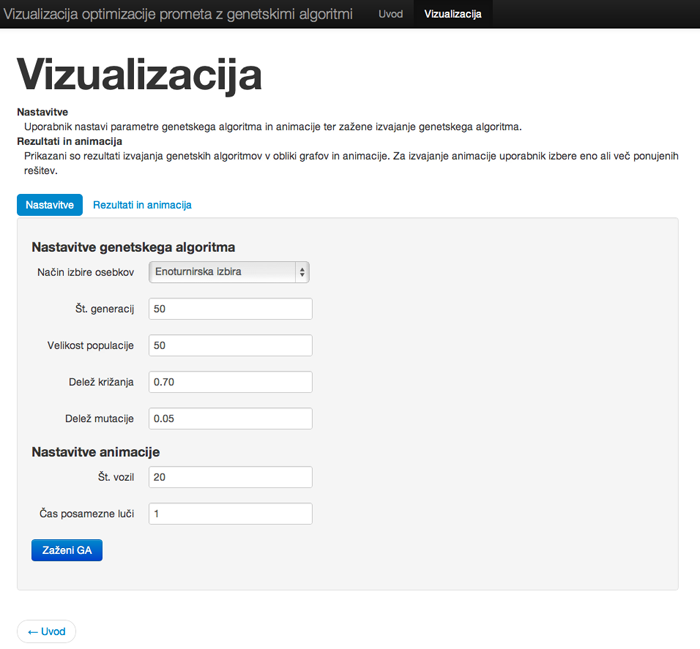
\includegraphics[scale=0.50]{nastavitev_parametrov.png}
\caption{Nastavitve za genetski algoritem in animacijo.}
\label{fig:vizualizacija-nastavitev parametrov}
\end{figure}

\begin{figure}
\centering
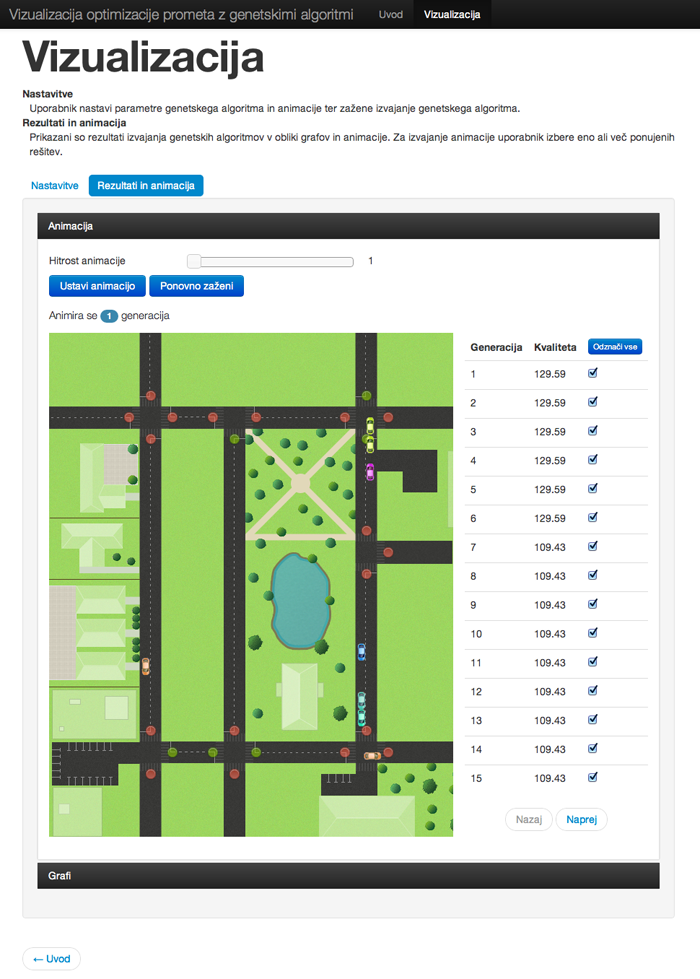
\includegraphics[scale=0.50]{rezultati.png}
\caption{Animacija rezultatov}
\label{fig:vizualizacija-rezultati}
\end{figure}

Po koncu izvajanja so uporabniku ponujeni rezultati v obliki grafov in animacije. Uporabnik izbere re\v sitve, ki jih \v zeli animirati. Re\v sitve so urejene od najslab\v se do najbolj\v se. Animacijo lahko ustavlja in ponovno za\v zene. Slika \ref{fig:vizualizacija-rezultati} prikazuje izbiro re\v sitev, kontrolne gumbe in izvajanje animacije.


\subsection{Animacija}
Animacija se izvaja v t.i. zanki igre (ang. game loop). Naloga zanke je izrisovanje in posodabljanje parametrov objektov, ki jih izrisuje. Zanka igre se mora izvajati dovolj hitro, da je animacija teko\v ca. \v Clovesko oko lahko zazna med 10 in 12 razli\v cnih slik na sekundo, kljub temu pa se obi\v cajno izris dela 50-krat na sekundo.

Pri animaciji smo izris 50-krat na sekundo dosegli tako, da ga delamo na 20 ms. V Javascriptu obstaja metoda \verb+setInterval(funkcija(), cas)+, ki na vsakih \verb+cas+ sekund pokli\v ce metodo \verb+funkcija()+. V na\v sem primeru je \verb+funkcija()+ metoda, ki poskrbi za izris in posodabljanje parametrov objekta, \verb+cas+ pa je nastavljen na 20 ms.

Pri animaciji se izrisujejo vozila in semaforji.  Za poenostavitev problema in  animacije smo vsem vozilom definirali isto hitrost premikanja in isti \v cas prihajanja. Vsa vozila vstopijo v animacijo ob \v casu 0.

\chapter{Tehnologije}
\label{ch3}
V tem poglavju opi\v semo tehnologije uporabljene pri razvoju vizualizacije, animacije in genetskega algoritma ter predstavimo orodje za t.i. dru\v zabno programiranje (ang. \textit{social coding}) GitHub.

\section{HTML}

HTML (\textit{HyperText Markup Language}) je glavni ozna\v cevalni jezik za prikazovanje spletnih strani in drugih vsebin v spletnem brskalniku.
%HTML je kratica za \textit{HyperText Markup Language} in je glavni ozna\v cevalni jezik za prikazovanje spletnih strani in ostalih informacij, ki jih lahko prika\v zemo v spletnem brskalniku. 
HTML je napisan v obliki elementov, sestavljenih iz zna\v ck (ang. \textit{tags}) zaprtih med znaka $< in >$. Zna\v cke najbolj pogosto nastopajo v obliki parov, npr. $<$h1$>$ in $<$/h1$>$. Obstajajo tudi prazne zna\v cke, ki nastopajo samostojno, npr. $<$img$>$. Prvo zna\v cko v paru imenujemo \textit{za\v cetna zna\v cka}, drugo pa \textit{kon\v cna zna\v cka}. Med te zna\v cke lahko oblikovalci spletnih strani dodajo besedilo, druge zna\v cke, komentarje in druge vsebine.

Privzete karakteristike vsakega HTML elementa so definirane v spletnem brskalniku, zato nekateri naprednej\v si spletni brskalniki vsebujejo zna\v cke, ki delujejo samo v dolo\v cenem brskalniku v ostalih pa ne.

Namen spletnega brskalnika je prebrati HTML dokument in ga pretvoriti v vidne in sli\v sne elemente spletne strani. Spletni brskalnik uporablja HTML zna\v cke za oblikovanje vsebine spletne strani in ne prikazuje HTML zna\v ck.

HTML predstavlja temelj spletnih strani in omogo\v ca uporabo slik in drugih objektov, vklju\v cenih v spletno stran, lahko pa se uporablja tudi za grajenje spletnih obrazcev. Omogo\v ca oblikovanje strukturiranih dokumentov z ozna\v cevanjem semantike besedila, npr. naslovi, odstavki, seznami, povezave, citati in drugi elementi. Omogo\v ca tudi vklju\v cevanje datotek drugih jezikov, ki vplivajo na prikaz spletne strani
\cite{wikipedia-html}.

\section{HTML5}
HTML5 je naslednja generacija HTML standarda, ki nadome\v s\v ca starej\v se standarde, kot so HTML 4.01, XHTML 1.0 in 1.1. Standard prina\v sa novosti, potrebne za moderne spletne aplikacije. Standard vklju\v cuje in definira mnoge lastnosti, ki so jih spletni razvijalci uporabljali \v ze leta, a niso bile vklju\v cene v katerega izmed standardov. HTML5 je prvi poskus formalno dokumentirati ``de facto`` standarde, ki jih spletni brskalniki podpirajo \v ze leta. Kot njegovi predhodniki je tudi HTML5 zasnovan platformno neodvisno.

HTML5 lahko uporabljamo in pregledujemo na poljubnem operacijskem sistemu in mobilni napravi. Uporabniki potrebujejo le moderen spletni brskalnik, le ti pa so brezpla\v cno na razpolago za prakti\v cno vse operacijske sisteme, npr. Google Chrome, Mozilla Firefox, Opera in Safari. Vsi na\v steti brskalniki podpirajo veliko HTML5 lastnosti, ne podpirajo pa vsi vseh. Odli\v cno podporo standardu HTML5 imajo tudi mobilni spletni brskalniki za mobilne naprave.

HTML5 je zasnovan za \v cim bolj\v so zdru\v zljivost z \v ze obstoje\v cimi spletnimi
brskalniki. Nove funkcionalnosti so zgrajene na starih in omogo\v cajo zdru\v zljivost
za starej\v se brskalnike. Obstoj posameznih funkcionalnost
HTML5 lahko ugotovite \v ze z nekaj vrsticami Javascripta.
\cite{html5}

HTML5 ne prina\v sa samo novih zna\v ck in novega standarda. Skupaj z razvojem naprednih spletnih brskalnikov omogo\v ca tudi lastnosti, ki so jih do sedaj imele le namizne aplikacije. Na\v stejmo nekaj glavnih lastnosti, ki jih danes omogo\v cajo spletni brskalniki
\cite{html5rocks}:

\begin{itemize}
\item \textbf{internet v brezpovezavnem na\v cinu (ang. offline web)},
\item \textbf{hranjenje podatkov v lokalni bazi brskalnika},
\item \textbf{povezljivost} - klepetanje v realnem \v casu, hitrej\v se igre, itd.,
\item \textbf{dostop do datote\v cnega sistema},
\item \textbf{semantika} - internacionalizacija, novi atributi za pomensko ozna\v cevanje vsebine, itd.,
\item \textbf{avdio/video},
\item \textbf{3d grafika},
\item \textbf{predstavitev} - 2D in 3D transformacije omogo\v cajo izdelavo bogatih uporabni\v skih vmesnikov,
\item \textbf{zmogljivost} - spletne aplikacije se lahko primerjajo z zmogljivostjo namiznih aplikacij.
\end{itemize}

Te lastnosti in druge, skupaj s standardom HTML5 definirajo splet kot platformo (ang. \textit{web platform}).

\section{CSS}
CSS je kratica za Cascading Style Sheet, kar bi v prevodu pomenilo predlogo, ki dolo\v ca izgled. Uporablja se za opisovanje izgleda dokumentov napisanih v ozna\v cevalnih jezikih. Najbolj pogosto se uporablja za opisovanje izgleda spletnih strani napisanih v HTML-ju in XHTML-ju, vendar lahko jezik uporabimo tudi v dokumentih XML, SVG in XUL. CSS specifikacije ureja World Wide Web Consortium (W3C).

CSS je prvenstveno namenjen lo\v cevanju vsebine od izgleda dokumenta. Taka lo\v citev lahko izbolj\v sa dostopnost vsebine, ponuja ve\v cjo fleksibilnost in nadzor nad specifikacjiami predstavitve, omogo\v ca deljenje istega stila \v cez ve\v c strani ter zmanj\v sa komplekstnost in ponavljanje stila v strukturiranih dokumentih. CSS omogo\v ca, da je ista stran predstavljena z ve\v c razli\v cnimi stili za razli\v cne zahteve izrisovanja (izris na zaslon, printanje, itd.). Lahko se uporabi za prikazovanje spletne strani na razli\v cnih resolucijah zaslona ali napravah.

CSS ima dolo\v ceno prioritetno shemo, da ugotovi, kateri stil uporabiti \v ce enemu elementu ustreza ve\v c pravil. V tako imenovani kaskadi so prioritete ali ute\v zi izra\v cunane in dodeljene pravilom tako, da so rezultati ujemanja pravil predvidljivi. To omogo\v ca oblikovalcem spletnih strani, da natan\v cno dolo\v cijo obliko vsebine spletne strani. Primer preprostega CSS stila za HTML zna\v cko $<$body$>$ je prikazan na sliki \ref{fig:css stil}
\begin{figure}
body\{\\
\hspace{6mm}{\textbf{font-family:} Arial;\\}
\hspace{6mm}{\textbf{font-size:} 11px;\\}
\hspace{6mm}{\textbf{color:} red;\\}
\}
\caption{CSS stil, ki nastavi barvo, velikost in tip pisave HTML zna\v cki $<$body$>$.}
\label{fig:css stil}
\end{figure}

\section{Javascript}
Javascript je programski jezik spletnega brskalnika. Bil je razvit v samo desetih dneh pri podjetju Netscape z namenom, da uporabnikom ponudijo lahko in prenosno razli\v cico Jave, ki bi izbolj\v sala uporabni\v sko izku\v snjo s spletno stranjo. 

Javascript je skriptni jezik, dinami\v cen in \v sibko tipiziran ter podpira ve\v c razli\v cnih vzorcev programiranja (objektno orientirano, funkcionalno, itd.). 

Najve\v c se jezik uporablja za izvajanje na strani klienta, implementiran kot del spletnega brskalnika za obogatitev uporabni\v skih vmesnikov in dinami\v cnih spletnih strani. 

Z razvojem vse hitrej\v sih navideznih strojev in programskih ogrodij za ta jezik, nara\v s\v ca tudi popularnost uporabe za stre\v zni\v ske spletne aplikacije. \v Ze leta 1994, kmalu po izdaji Javascript jezika, je isto podjetje izdalo \v se razli\v cico na voljo za stre\v znike. Eden popularnej\v sih okolij za razvoj stre\v zni\v skih spletnih aplikacij je orodje Node.js.

Javascript uporablja sintakso podobno programskemu jeziku C. Veliko imen in pravil poimenovanja spremenljivk ter funkcij je vzetih iz programskega jezika Java, vseeno pa sta tadva jezika nepovezana in imata popolnoma razli\v cno semantiko. Klju\v cni principi pri oblikovanju so bili vzeti iz Self in Scheme programskega jezika. 

\begin{figure}
\begin{lstlisting}
var factorial = function(n) {
    if (n === 0) {
        return 1;
    }
    return n * factorial(n - 1);
}
\end{lstlisting}
\caption{Primer Javascript kode za izra\v cun Fibonaccijevega zaporedja}
\label{fig:javascript primer}
\end{figure}

\section{GitHub}
\label{seq:github}
GitHub je spletna storitev za gostovanje programske opreme, ki uporablja za nadzor razli\v cic programske opreme Git kontrolni sistem. Git je distribuiran kontrolni sistem za nadzor razli\v cic programske opreme in sistem za upravljanje z izvorno kodo.

GitHub uporabnikom ponuja pla\v cljive pakete za privatne projekte in zastonjski paket za odprtokodne projekte. V Juliju 2011 je podjetje dobilo investicijo v vrednosti 100 miljonov ameri\v skih dolarjev od znane investicijske hi\v se Andreessen Horowitz.

GitHub ponuja funkcionalnosti socialnega omre\v zja, kot so: viri (ang. \textit{feeds}), spremljevalci (ang. \textit{followers}) in graf omre\v zja za prikaz, koliko razvijalcev trenutno sodeluje pri razvoju projekta.
\cite{wikipedia-github}

\chapter{Rezultati}
\label{ch4}

V tem poglavju predstavimo rezultate izvajanja genetskih algoritmov za vsako metodo izbire posebej in na koncu podamo ugotovitve.

\section{Proporcionalna izbira}
Proporcionalno izbiro smo zagnali s parametri iz razdelka \ref{seq:nastavitve parametrov}. Slika \ref{res:proporcionalna izbira} prikazuje konvergenco kvalitete najbolj\v sega osebka. Na za\v cetku se kvaliteta zelo hitro izbolj\v sa (s 3.40 pade na 3.00), potem pa se izbolj\v suje po\v casneje. V\v casih se celo nekaj generacij ne izbolj\v sa, npr. od 60 do 100 generacije. 

Genetski algoritem smo zagnali z manj\v sim \v stevilom generacij in pove\v canim dele\v zom kri\v zanja (0.80). Dobili smo bolj\v so re\v sitev, kot s prej\v snimi nastavitvami. Kvaliteta je konvergirala k vrednosti 2.19. Za proporcionalno izbiro lahko re\v cemo, da v splo\v snem potrebujemo manj generacij, vendar se moramo pri tem zavedati, da lahko na ta ra\v cun dobimo slab\v so re\v sitev.

\begin{figure}
\centering
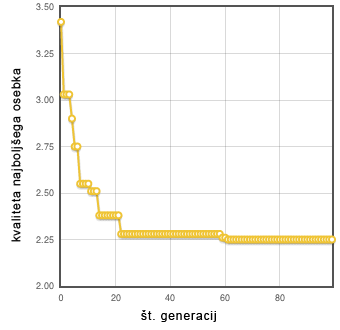
\includegraphics[scale=0.70]{prop_izbira.png}
\caption{Rezultati izvajanja genetskega algoritma z nastavitvami iz razdelka \ref{seq:nastavitve parametrov} in proporcionalno izbiro.}
\label{res:proporcionalna izbira}
\end{figure}

\section{Enoturnirska izbira}
Pri metodi enoturnirske izbire smo osebke izbirali na dva na\v cina, z vra\v canjem in brez vra\v canja. V nadaljevanju so predstavljeni rezultati obeh izvajanj.

\subsubsection{Izbira osebkov brez vra\v canja}
Enoturnirsko izbiro smo najprej zagnali z nastavitvami iz razdelka \ref{seq:nastavitve parametrov}, osebke pa smo izbirali brez vra\v canja. Rezultate prikazuje slika \ref{fig1}. Opazimo, da kvaliteta najbolj\v sega osebka zelo niha, na zacetku sko\v ci z 2.75 na 2.88. Kljub nihanju se \v v kak\v sni generaciji kvaliteta izbolj\v sa. Za kon\v cno re\v sitev vrnemo re\v sitev z najbolj\v so kvaliteto, t.j. to\v cka z najmanj\v so vrednostjo na grafu (2.45 - rde\v ca to\v cka na sliki \ref{fig1}).

\begin{figure}
\centering
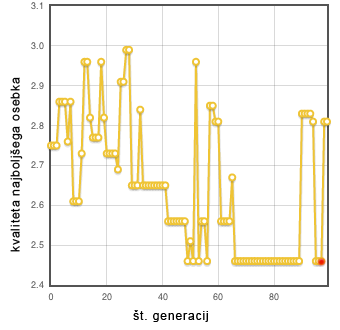
\includegraphics[scale=0.70]{enotur_mut_brez_vrac.png}
\caption{Rezultati izvajanja genetskega algoritma z nastavitvami iz razdelka \ref{seq:nastavitve parametrov} z enoturnirsko izbiro, mutacijo in brez vra\v canja.}
\label{fig1}
\end{figure}

Genetski algoritem smo nato pognali z istimi nastavitvami le, da smo dele\v z mutacije nastavili na 0.
Rezultati so prikazani na sliki \ref{fig2} na kateri opazimo, da kvaliteta \v se vedno niha, a manj in se \v cez generacije izbolj\v suje. Za kon\v cno re\v sitev vrnemo re\v sitev z najbolj\v so oceno (2.47 - rde\v ca to\v cka na sliki \ref{fig2})

\begin{figure}
\centering
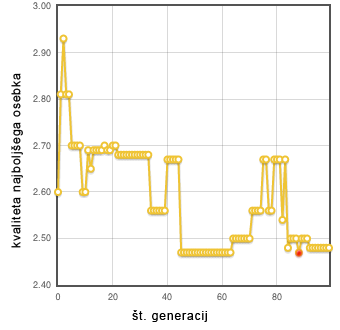
\includegraphics[scale=0.70]{enotur_brez_mut_brez_vrac.png}
\caption{Rezultati izvajanja genetskega algoritma z nastavitvami iz razdelka \ref{seq:nastavitve parametrov} z enoturnirsko izbiro, brez mutacije in brez vra\v canja.}
\label{fig2}
\end{figure}

\subsubsection{Izbira osebkov z vra\v canjem}
Enoturnirsko izbiro smo nato spremenili tako, da osebke za reprodukcijo izbira z vra\v canjem. Podobno kot prej smo genetski algoritem pognali z mutacijo in brez mutacije. Slika \ref{enotur brez mutacije} prikazuje, da so re\v sitve brez mutacije neuporabne.

\begin{figure}
\centering
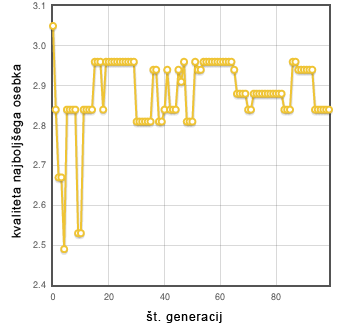
\includegraphics[scale=0.70]{enotur_brez_mutacije.png}
\caption{Rezultati izvajanja genetskega algoritma z nastavitvami iz razdelka \ref{seq:nastavitve parametrov} z enoturnirsko izbiro, brez mutacije in z vra\v canjem.}
\label{enotur brez mutacije}
\end{figure}

Slika \ref{fig3} prikazuje rezultate izvajanja genetskega algoritma z dele\v zom mutacije enakemu tistemu iz razdelka \ref{seq:nastavitve parametrov}. Vidimo, da kvaliteta \v se vedno niha vendar \v se cez generacije izbolj\v suje, splo\v sno pa so kvalitete slab\v se (najbolj\v sa ima vrednost 2.8). Bolj\v se kvalitete (slika \ref{fig4}) dose\v zemo \v ce nastavimo dele\v z mutacije na vrednost 0.10 (najbolj\v sa ima vrednost 2.45) . Dele\v z mutacije ne smemo nastaviti na preveliko vrednost, saj potem dobimo slab\v se rezultate.

\begin{figure}
\centering
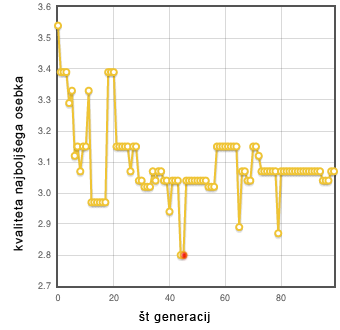
\includegraphics[scale=0.70]{enotur_vrac_mut1.png}
\caption{Rezultati izvajanja genetskega algoritma z nastavitvami iz razdelka \ref{seq:nastavitve parametrov} z enoturnirsko izbiro, z mutacijo 0.05 in z vra\v canjem.}
\label{fig3}
\end{figure}

\begin{figure}
\centering
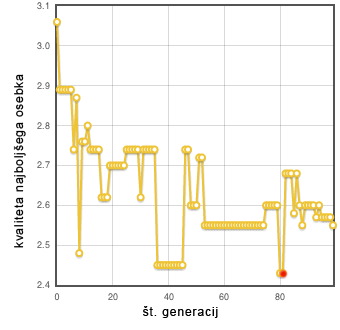
\includegraphics[scale=0.70]{enotur_vrac_mut2.png}
\caption{Rezultati izvajanja genetskega algoritma z nastavitvami iz razdelka \ref{seq:nastavitve parametrov} z enoturnirsko izbiro, z mutacijo 0.10 in z vra\v canjem.}
\label{fig4}
\end{figure}

\section{Stohasti\v cno univerzalno vzor\v cenje}
Stohasti\v cno univerzalno vzor\v cenje smo zagnali z nastavitvami iz razdelka \ref{seq:nastavitve parametrov}. Na sliki \ref{fig5} opazimo, da kvaliteta zelo hitro konvergira. Z ve\v canjem mutacije je kvaliteta konvergirala po\v casneje in k bolj\v sim re\v sitvam.

\begin{figure}
\centering
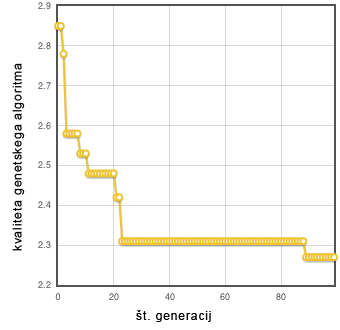
\includegraphics[scale=0.70]{graph7.png}
\caption{Rezultati izvajanja genetskega algoritma z nastavitvami iz razdelka \ref{seq:nastavitve parametrov} in metodo stohasti\v cnega univerzalnega vzor\v cenja.}
\label{fig5}
\end{figure}

\section{Ugotovitve}

Primerjava kvalitet re\v sitev vseh treh metod izbire poka\v ze, da najslab\v se rezultate daje metoda enoturnirske izbire. Preostali dve metodi dajeta bolj\v se rezultate in potrebujeta manj\v se \v stevilo generacij za konvergenco, zato lahko trdimo, da enoturnirska izbira ni primerna za re\v sevanje takega problema. 

Rezultati izvajanja genetskega algoritma so pokazali, da je kvaliteta re\v sitev precej odvisna od za\v cetne populacije.
\v Casovna zahtevnost vseh metod izbire je precej\v sna, za najpo\v casnej\v so pa se izka\v ze metoda stohasti\v cnega univerzalnega vzor\v cenja.

\chapter{Zaklju\v cek}
V diplomski nalogi predstavimo delovanje genetskih algoritmov in problem usmerjanja prometa.
Predstavimo na\v s pristop k re\v sevanju problema in ga formaliziramo. Predstavimo implementacijo genetskih operatorjev in tehnologije uporabljene pri tem. Z grafi predstavimo rezultate izvajanja genetskih algoritmov z razli\v cnimi nastavitvami in ugotovitve.

\subsubsection{Mo\v zne izbolj\v save}

Genetske algoritme je zaradi posnemanja evolucije enostavno paralelizirati. Izbolj\v sava, ki bi mo\v cno izbolj\v sala hitrost izvajanja genetskega algoritma, je paralelizacija ra\v cunanja kvalitete ene re\v sitve. To bi lahko naredili tako, da bi imeli en nadrejeni proces, ki bi hranil populacijo in izvajal genetske operatorje, osebke pa bi poslal podrejenim procesom. Edina naloga podrejenih procesov bi bila ra\v cunanje kvalitete ene re\v sitve
\cite{http://tracer.uc3m.es/tws/cEA/documents/cant98.pdf}.

Za doseganje bolj\v sih re\v sitev bi lahko na mestih, kjer se kvaliteta najbolj\v sega osebka nekaj generacij ne izbolj\v suje, pove\v cali mutacijo. Tako bi dobili nove osebke s potencialno novo informacijo.

K re\v sevanju problema optimizacije prometa bi lahko pristopili druga\v ce. Mo\v zen pristop je, da bi sku\v sali optimizirati \v case na semaforjih glavne ceste s pritoki. Za vozila na glavni cesti bi \v zeleli ujeti zeleni val, vozila s stranskih cest pa bi predstavljala motnje. \v Case na semaforjih bi sku\v sali optimizirati tudi za vozila, ki prihajajo s stranskih cest, vendar bi imeli semaforji na kri\v zi\v s\v cu med glavno cesto in stransko manj\v so te\v zo. Na ta na\v cin bi se na glavni cesti s\v casoma za\v celi delati prometni zastoji in bi vozila potrebovala dlje \v casa za potovanje do cilja. 
 

 
\begin{thebibliography}{99}
\bibitem{inteligentni sistemi} Igor kononenko, Marko Robnik \v Sikonja, \textit{Inteligentni sistemi}, Zalo\v zba FE in FRI, pogl. 12, 2010.
\bibitem{he12-aes.pdf} Jiajia He, Zaien Hou, ``Ant colony algorithm for traffic signal timing optimization``, \textit{Advances in Engineering Software}, \v st. 43, zv. 1, str.  14-18, 2012.
\bibitem{html5} Ciril Bohak, ``HTML5``, str. 3, 2010. Dostopno na:\\
http://atlas.fri.uni-lj.si/html5-primeri/HTML5-Script.pdf
\bibitem{sarmady} Siamak Sarmady, ``An Investigation on Genetic Algorithm Parameters``. Dostopno na:\\ http://sarmady.com/siamak/papers/genetic-algorithm.pdf
\bibitem{wikipedia genetski algoritmi} (2012) Genetic algorithm from Wikipedia, the free encyclopedia. Dostopno na:\\
http://en.wikipedia.org/wiki/Genetic\_algorithm
\bibitem{aijunkie} (2012) Genetic Algorithms in Plain English. Dostopno na:\\
http://www.ai-junkie.com/ga/intro/gat1.html
\bibitem{github-stohasticno} (2012) Izvorna koda stohasti\v cnega univerzalnega vzor\v cenja v Javi. Dostopno na:\\
https://github.com/dwdyer/watchmaker/blob/master/framework/src/\\
java/main/org/uncommons/watchmaker/framework/selection/\\
StochasticUniversalSampling.java
\bibitem{wikipedia-html} (2012) HTML from Wikipedia, the free encyclopedia. Dostopno na:\\
http://en.wikipedia.org/wiki/Html
\bibitem{html5rocks} (2012) HTML5 Rocks. Dostopno na:\\
http://www.html5rocks.com/
\bibitem{wikipedia-github} (2012) GitHub from Wikipedia, the free encyclopedia. Dostopno na:\\
http://en.wikipedia.org/wiki/Github
\bibitem{slika ruletno kolo}(2012) Roulette wheel selection. Dostopno na:\\
http://www.edc.ncl.ac.uk/highlight/rhjanuary2007g02.php/
\bibitem{izvorna koda}(2012) Izvorna koda aplikacije. Dostopno na:\\
https://github.com/Ivansek/thesis
\end{thebibliography}
\end{document}

